\documentclass[letterpaper, 11pt]{article}
\usepackage{authblk}	% For nice author-affil lists
\usepackage{graphicx}	% For figures
\usepackage{natbib}	% For citet and citep
\usepackage{amsmath}	% for \iint
\usepackage{bbm}	% for blackboard bold numbers
\usepackage[left=3cm,top=3cm,right=3cm]{geometry}

\renewcommand{\topfraction}{0.85}
\renewcommand{\textfraction}{0.1}
\parindent=0cm
\newcommand{\yy}{\mathbf{y}}

\title{Reliable Inferences from Simply Parameterised Models}

\author[1,2]{Brendon J. Brewer}
\author[3]{Geraint~F.~Lewis}
\author[4]{Ross Fadely}
\affil[1]{\small Dept. of Physics, University of California, Santa Barbara, CA 93106, USA}
\affil[2]{Department of Statistics, University of Auckland, Private Bag 92019, Auckland, New Zealand
}
\affil[3]{Sydney Institute for Astronomy, School of Physics, The University of Sydney, A28, Sydney, 2006, Australia}
\affil[4]{Department of Astronomy, Haverford College, 370 Lancaster Ave., Haverford, PA 19041 USA}

\begin{document}

\date{\today}

\maketitle

\begin{abstract}
We discuss the practical use of simply parameterised models in Bayesian data analysis, particularly in astronomy.
The use of simply parameterised models is problematic when they are fit to large, informative data sets, resulting in unrealistically small uncertainties on inferences. In common parlance, the formal statistical errors may be small, but the systematic errors are often large and in many cases, difficult to quantify at all. In principle, the best solution to this problem is to develop more realistic complex models that accurately describe our prior beliefs. However, this is often infeasible in practice, due to computational limitations and the difficulty of defining satisfactory prior distributions over high dimensional spaces. As a pragmatic alternative, we show that it is possible to reinterpret the use of simple models in a way that avoids the problem of overconfident
inferences. The key idea is to weaken the connection between the parameters and the data that is assumed in the prior probabilities. This weakening can be implemented straightforwardly using the Nested Sampling algorithm.
\end{abstract}

\section{Introduction}

Bayesian Inference is a powerful framework for modelling uncertainty that has
been successfully applied in many scientific fields. The basic idea
is that we can model the degree of plausibility of a hypothesis $H$ by a real
number in $[0, 1]$, and that these numbers should be manipulated according to
the rules of probability theory. If we are initially uncertain about some
hypothesis $H$, we model this as a {\it prior probability} $P(H)$. If some other
hypothesis $D$ is discovered to be true, the plausibility of $H$ is updated to
the {\it posterior probability} using Bayes' rule:
\begin{equation}
P(H|D) = \frac{P(H)P(D|H)}{P(D)}
\end{equation}

One common application of Bayesian Inference is for parameter estimation.
Suppose there is some quantity $\theta$ that is unknown. Initially, we describe
our uncertainty by a prior probability distribution $p(\theta)$. We also know about some
observation or experiment that will yield data $D$ that will provide some
information about $\theta$. We describe our knowledge about this process by a 
set of conditional probability distributions $p(D|\theta)$. Then, once a specific data set
$D_{\rm obs}$ has been observed, we update our state of knowledge about $\theta$
to the {\it posterior distribution}:
\begin{equation}
p(\theta | D) \propto p(\theta) p(D|\theta)|_{D=D_{\rm obs}}
\end{equation}
The various terms in this equation have the following names and meanings.

\begin{itemize}
\item $p(\theta|D)$ is the {\it posterior distribution}
for the parameters, and is usually the goal of the calculation. It describes our
knowledge and remaining uncertainty about $\theta$ after taking into account the data. \\

\item $p(\theta)$ is the {\it prior distribution}, a probability distribution
over possible values for $\theta$ that describes our uncertainty about
$\theta$ before taking into account the data. In many applications, this is a broad
probability distribution describing a large amount of uncertainty. \\

\item $p(D|\theta)$ is a function of
both $\theta$ and $D$ and is sometimes referred to as the {\it sampling distribution}.
Another name is the generative model. 
The sampling distribution $p(D|\theta)$ is a set of probability distributions,
one for each value of $\theta$, and describe our prior information about how the data are connected to the parameters \citep{2008arXiv0808.0012C}. In particular, it is the probability distribution
for the data we might observe, {\it if} we knew the true value of the parameters
$\theta$, as a function of $\theta$.

\item $p(D|\theta)|_{D = D_{\rm obs}}$ is called the {\it likelihood function}.
It is obtained from the sampling distribution, with the actual data substituted in,
and is therefore a function of $\theta$ only. It describes the effects of the actual data
set that was observed on our beliefs about $\theta$: values of $\theta$ with a high
likelihood predicted the data well and will have their probability upweighted
in the posterior distribution.
\end{itemize}

\begin{figure*}
\begin{center}
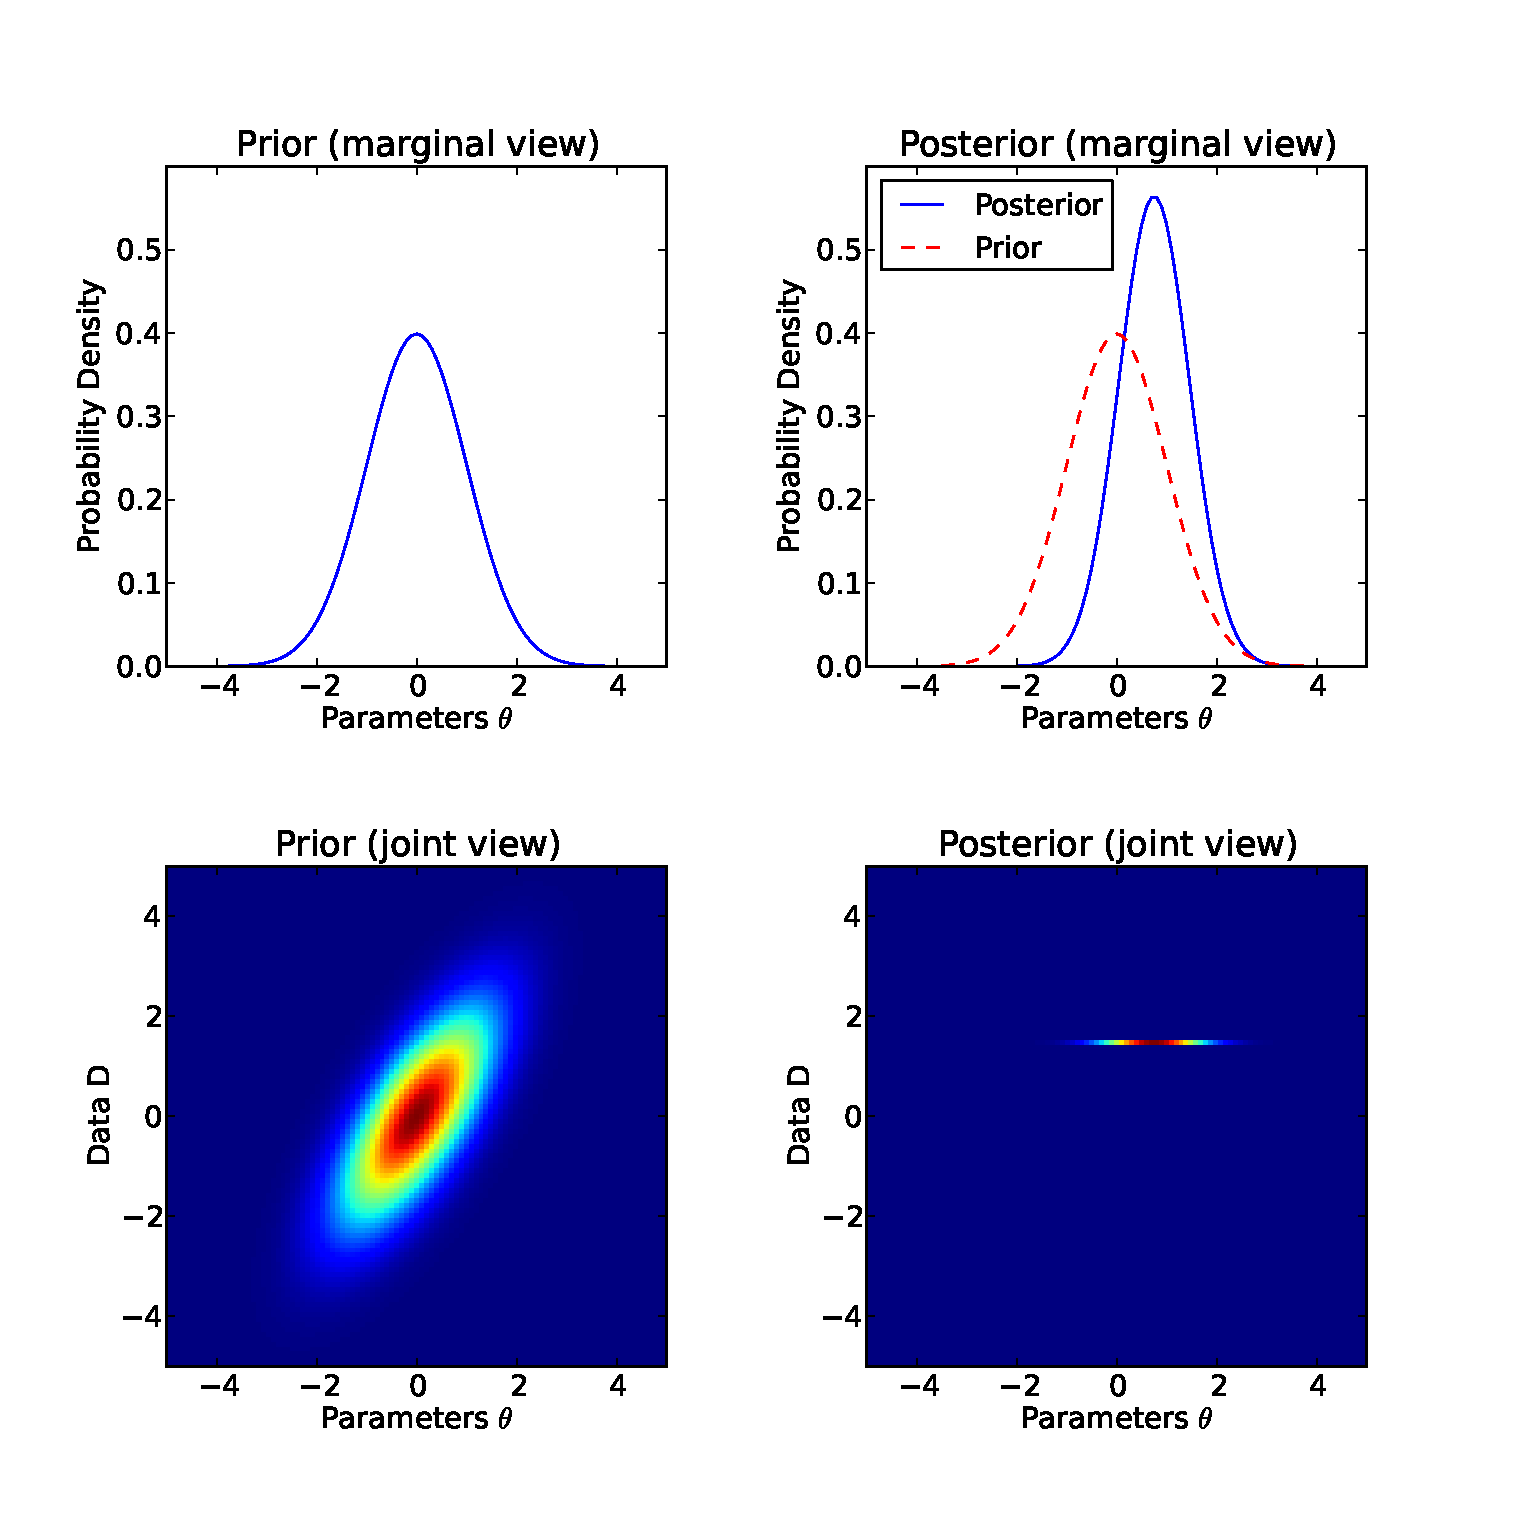
\includegraphics[scale=0.5]{joint_marginal.eps}
\end{center}
\end{figure*}

When the number of parameters being inferred is 3 or greater, enumeration of
all possible values becomes computationally prohibitive. In this situation,
Markov Chain Monte Carlo (MCMC) methods are commonly used to produce samples
drawn from the posterior distribution. These samples can then be used to view
the marginal distribution for any particular parameter(s) of interest.
In addition, if the
samples are viewed as a movie, they can give the viewer an intuitive sense of
the uncertainty in the determination of the parameters: any feature of the
models that varies between movie frames is a conclusion that is uncertain, and any
feature that is common to all frames in the movie is a feature that has a high
posterior probability.

{\bf Discuss the various attempts at robustness/model checking/elicitation and that stuff}

\section{Two Kinds of Model}
In this paper we consider two general categories of models that can be fit to
data. The first of these we will call ``simply-parameterised'' models.

\subsection{Simply-Parameterised Models}
Simply-parameterised models, which are also
commonly known as parametric models, are in widespread use for a number of reasons.
Firstly, they are easy to implement in software, and sometimes analytical
solutions are available for the inference of their parameters from data.
Secondly, their parameters usually have simple meanings that are easy to interpret.
This property makes communication easy, as well as making it straightforward to
make uncontroversial prior probability
assignments to the possible values of the parameters. Finally, when the inference
is done computationally, the MCMC methods tend to work very well.

\subsection{Complex Models}
The second category of models we consider are ``complex'' models. These tend to
be much more flexible and contain large numbers of unknown parameters. Complex
models are often incorrectly referred to as nonparametric models. A better term
would be flexible models or free-form models. The primary advantage of complex models is realism. The universe is not
simple place, and it is rare that a physical situation can be described accurately
by a simply-parameterised model which is often a simple mathematical formula.

\section{An Example: Fitting an Emission Line}
Throughout this paper we will use a simple example of fitting an emission line
to noisy data to explore the properties of simply parameterised models. The
simulated data was generated from the following complex model:
\begin{eqnarray}
\mathcal{M}_0(x) \propto 3\exp\left[-\frac{1}{2}\left(\frac{x}{0.3}\right)^2\right]
+ \exp\left[-\frac{1}{2}\left(\frac{x - 1}{1}\right)^2\right]
+ 5\exp\left[-\frac{1}{2}\left(\frac{x + 1}{0.5}\right)^2\right]
%M = 3*exp(-0.5*(x/0.3)**2) + exp(-0.5*(x-1.)**2) + 5*exp(-0.5*((x+1)/0.5)**2)
\end{eqnarray}
The fluxes were evaluated at $x$-values ranging from $-10$ to $10$ in steps
of $0.001$, and then normalised to sum to 1:
\begin{eqnarray}
\sum_{i=1}^N \mathcal{M}_0(x_i) &=& 1.
\end{eqnarray}
To simulate noise in the measurement process, errors $\{\epsilon_i\}$ were added, generated
independently from a normal distribution with mean 0 and standard deviation
$\sigma = 3 \times 10^{-4}$.
This produces noisy data $\mathbf{y} = \{y_1, y_2, ..., y_N\}$:
\begin{eqnarray}
\begin{array}{lccr}
y_i = \mathcal{M}_0(x_i) + \epsilon_i, & & & \epsilon_i \sim \mathcal{N}(0, \sigma^2).
\end{array}
\end{eqnarray}


\subsection{The Simply-Parameterised Model}
The model for the shape of the line is:
\begin{eqnarray}
\mathcal{M}(x; A, c, w) &=&
A\exp
\left[
-\frac{1}{2w^2}
\left(x - c\right)^2
\right]
\end{eqnarray}
where $A$ is the peak amplitude, $c$ is the central position of the line
and $w$ is the line width. To infer the parameters $\{A, c, w\}$ from some data
$\yy$, we will use Bayes' rule:
\begin{eqnarray}
p(A, c, w | \yy) \propto p(A, c, w)p(\yy | A, c, w).
\end{eqnarray}
To proceed, we just need to define the prior and the sampling distribution.

\subsection{The Sampling Distribution}
We will assume that the data are simply noisy measurements of the true line shape
$\mathcal{M}(x)$ at a finite number of $x$-values.
The sampling distribution, aka the probability distribution for the data $\yy$ given
the parameters, is simply a normal/gaussian distribution. Note that the
gaussian error assumption should be distinguished from the assumption of a gaussian
shape for the emission line.

\begin{eqnarray}
p(\yy|A, c, w) &=& \prod_{i=1}^N
\frac{1}{\sigma\sqrt{2\pi}}
\exp
\left[
-\frac{1}{2\sigma^2}\left(y_i - \mathcal{M}(x_i; A, c, w)\right)^2
\right] \\
&\propto& \exp\left[-\frac{1}{2\sigma^2}\sum_{i=1}^N\left(y_i - \mathcal{M}(x_i; A, c, w)\right)^2\right] \\
&\propto& \exp\left[-\frac{1}{2}\chi^2\right].
\end{eqnarray}


\begin{figure*}
\begin{center}
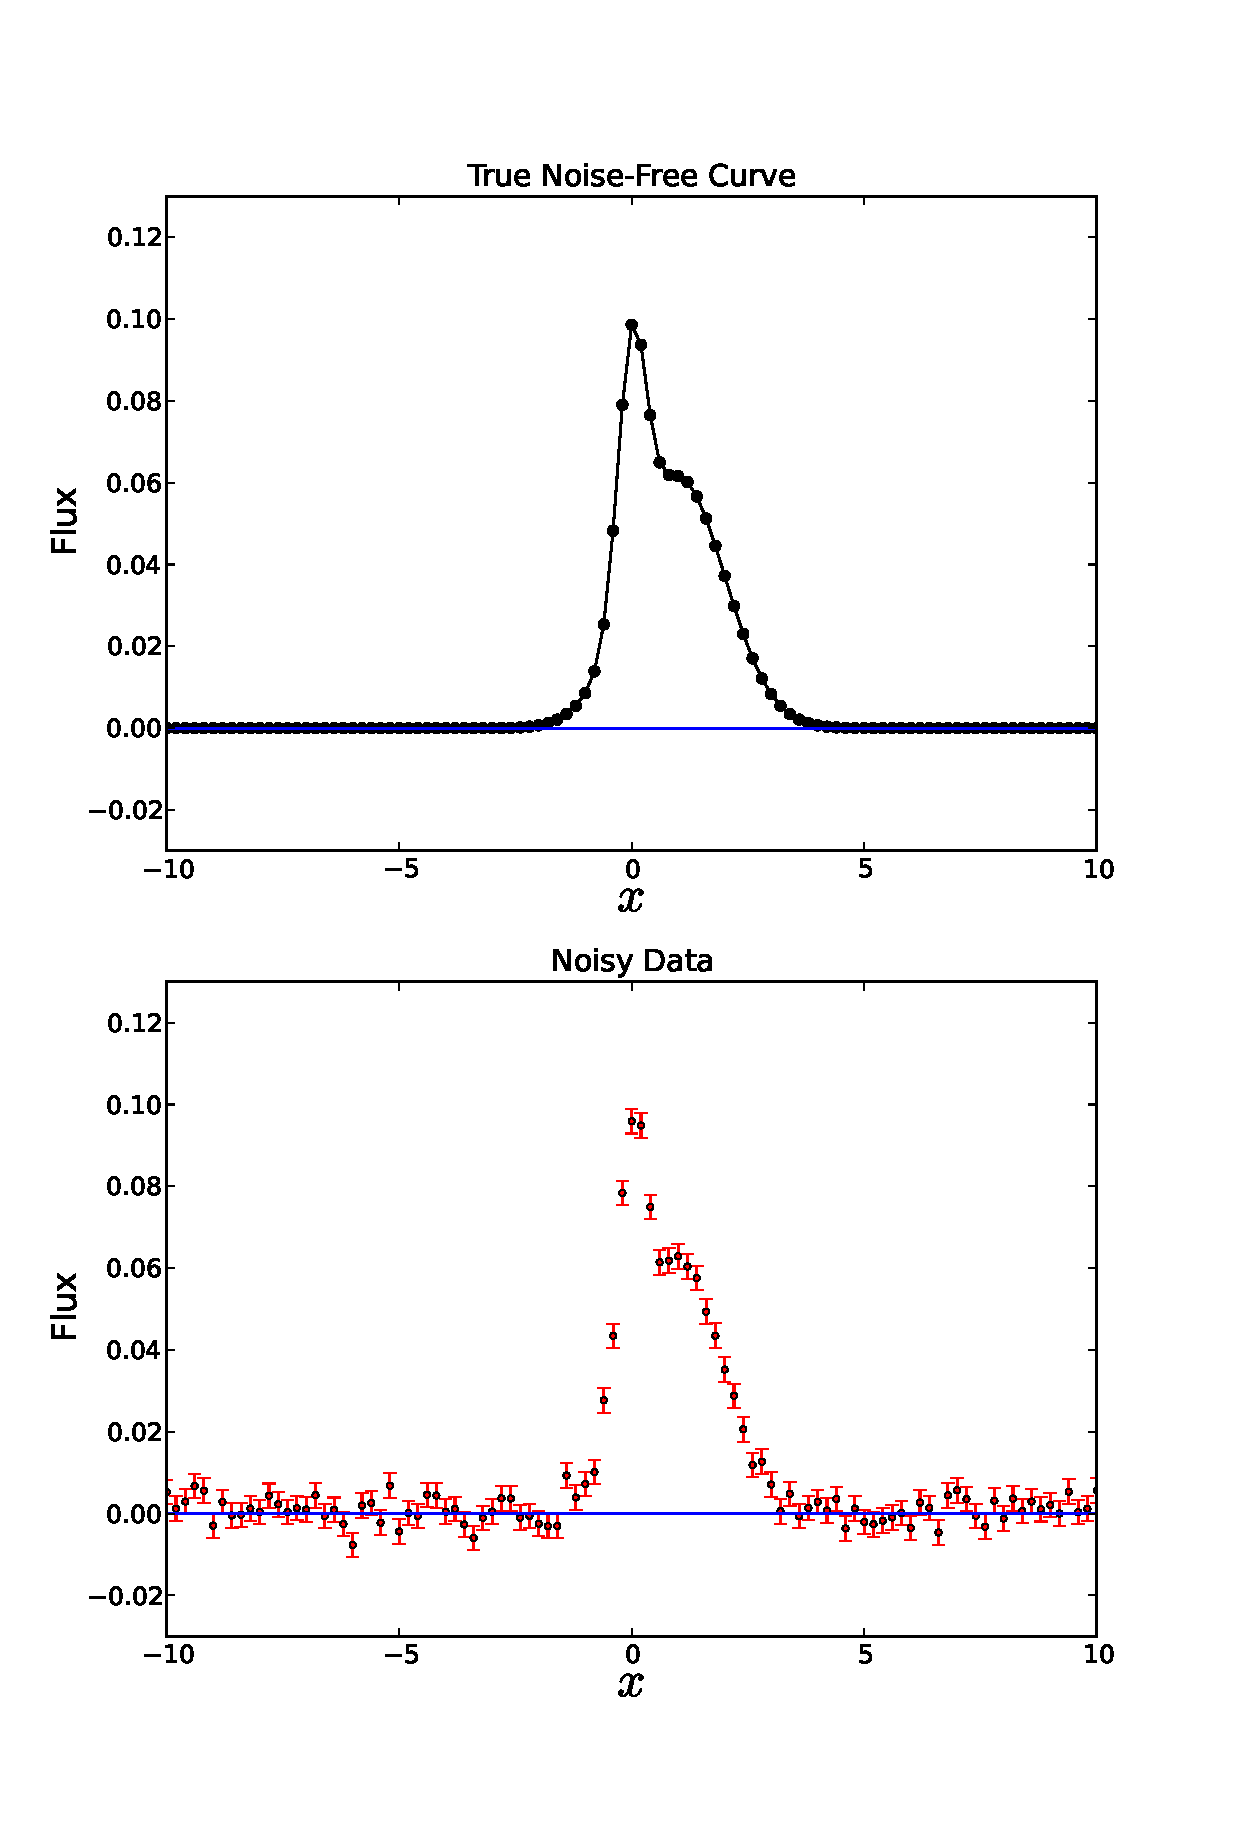
\includegraphics[scale=0.5]{emission_line.eps}
\end{center}
\end{figure*}

\section{The Failure of Simply Parameterised Models}
\begin{itemize}
\item Easy to implement \\
\item Computationally fast to get inferences - therefore can be applied on a large scale, e.g. to large samples of objects. \\
\item Easy to assign non-controversial priors over low dimensional parameter spaces \\
\end{itemize}

\section{Problems with Simply Parameterised Models}
\begin{itemize}
\item They are usually false, i.e. poor models of our actual prior beliefs. \\
\item Conditional on the simple model, you get error bars that are much too small. Small error bars on the parameters may not matter so much (since the parameters don't ``exist'' anyway), but the inferences on quantities that do ``exist'' (e.g. total flux) will still be overconfident. \\
\end{itemize}

\section{Re-Interpreting Simply Parameterised Models}

\begin{itemize}
\item Describe the hypothetical process of acknowledging the complex reality, yet describing (summarising) it by fitting a simple model to the complex one. \\
\item Show some examples of this - complex curves being approximated by lines with least squares, complex density profiles (1-D and 2-D) being fit by simple density profiles by maximising some kind of entropy.
\item Mention/derive that in the special case of fitting a complex density profile with a Gaussian, the variance(s) of the Gaussian gives the actual moment(s) of the complex profile
\item Describe how fitting a simple model can be interpreted as attempting to infer the parameters of the summarising simple model, and that therefore the parameter space is completely legitimate - it's the likelihood function that is now wrong. Data = model predictions + noise breaks down, it should be Data = simple model predictions + complexity perturbations + noise
\item Describe why qualitatively, the likelihood function should now be ``weaker'' than before
\item Describe why the old likelihood function is still (often) a good hill to climb
\end{itemize}

\begin{figure*}
\begin{center}
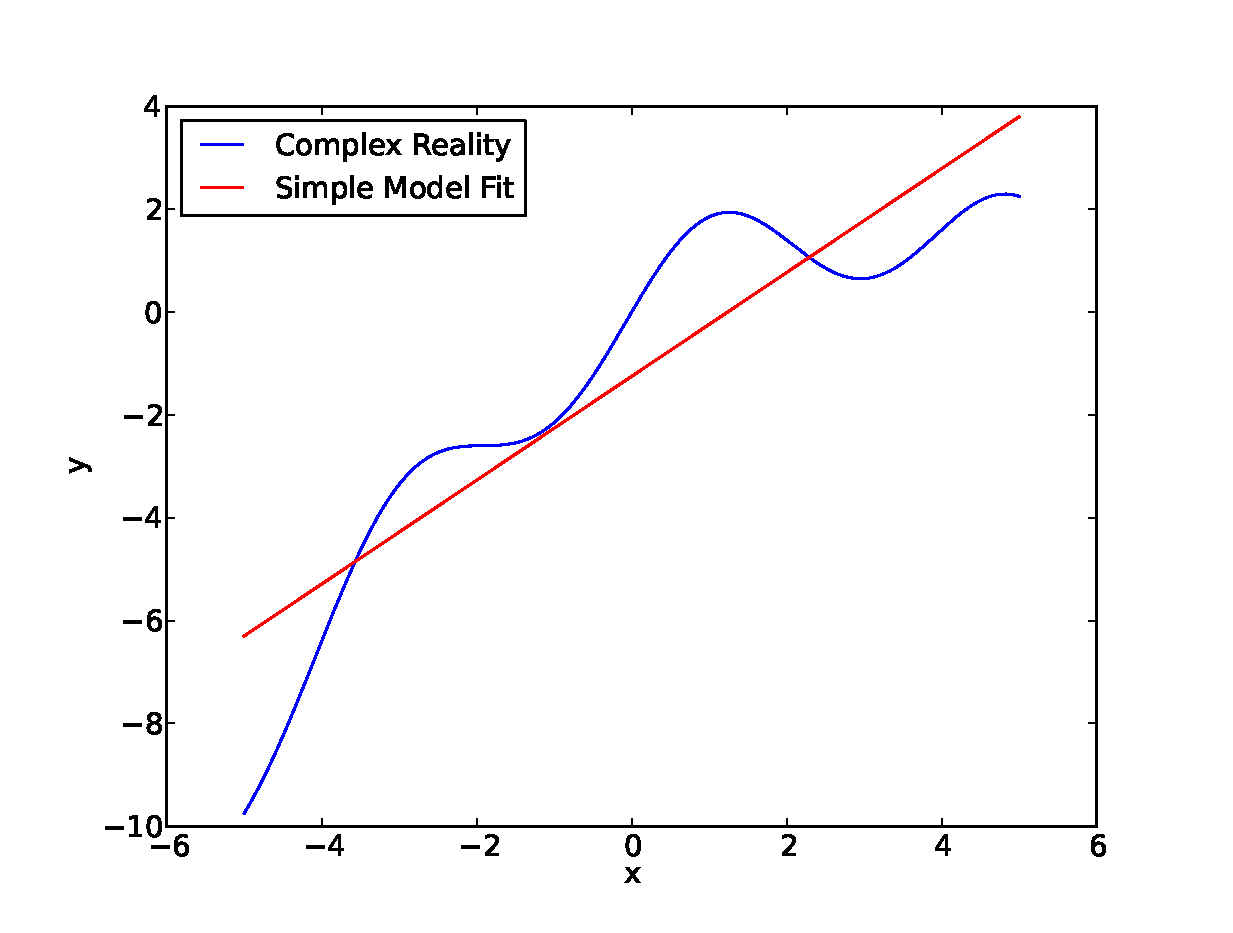
\includegraphics[scale=0.25]{simple_complex1.eps}
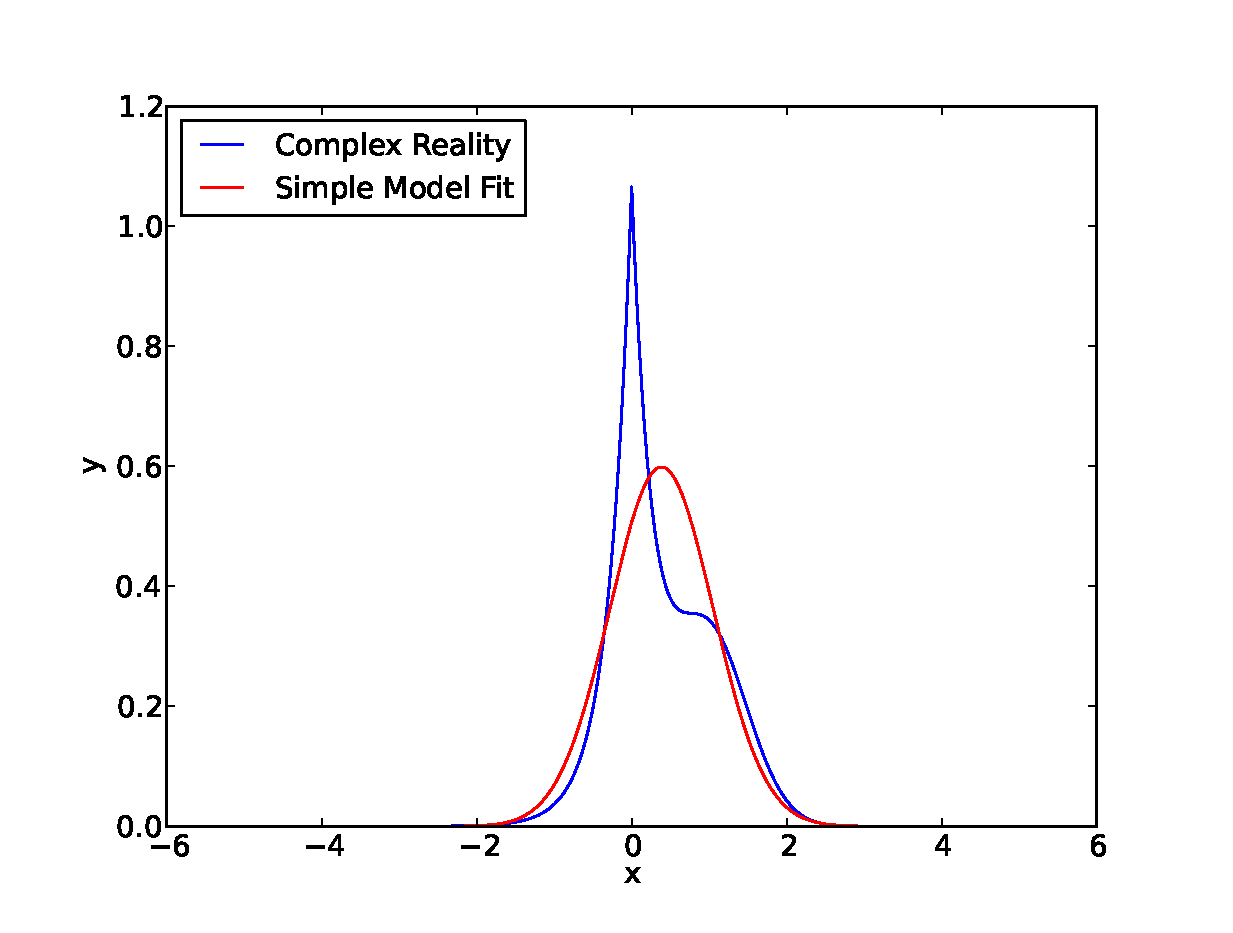
\includegraphics[scale=0.25]{simple_complex2.eps}
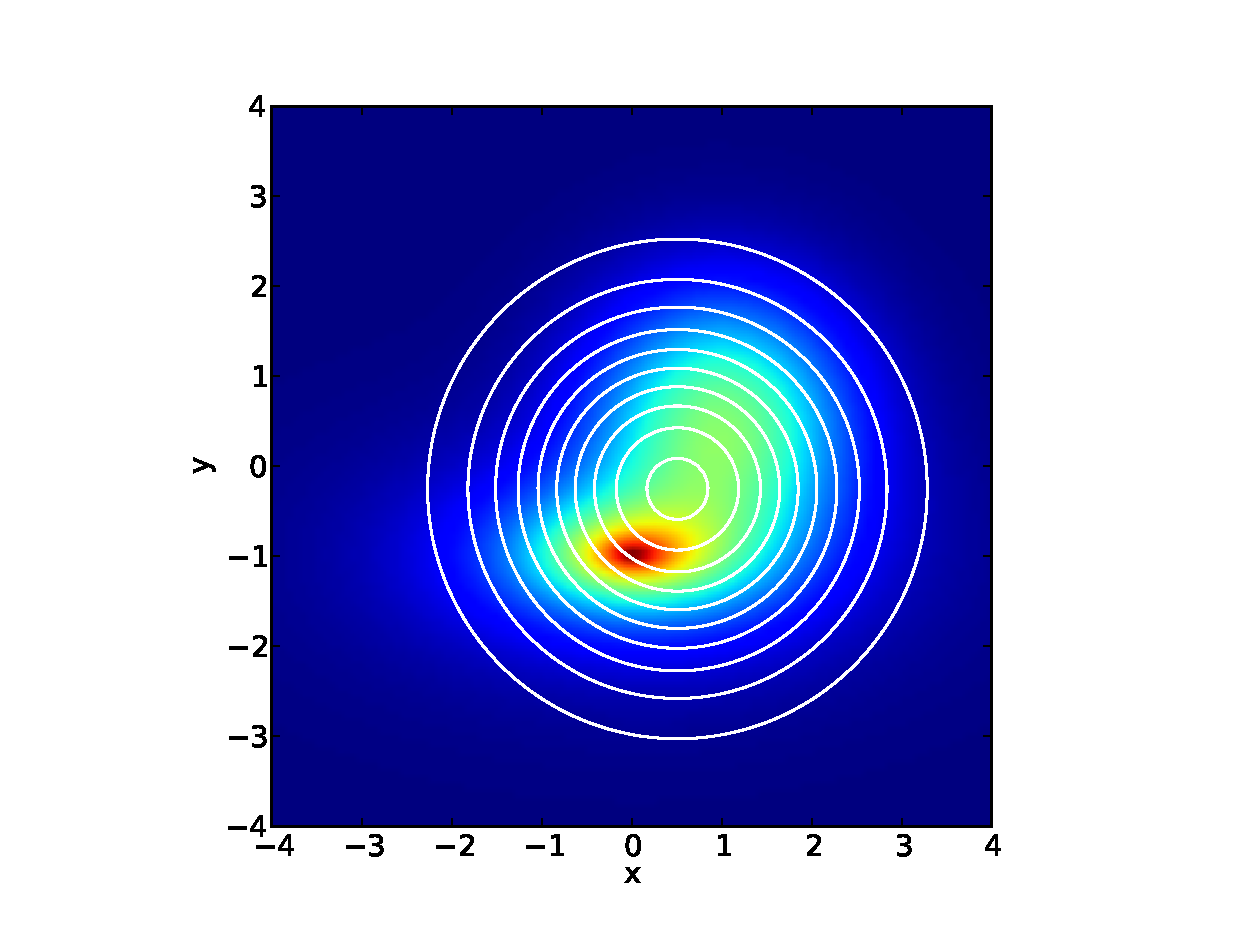
\includegraphics[scale=0.25]{simple_complex3.eps}
\end{center}
\end{figure*}

\section{Implementation with Nested Sampling}
\begin{itemize}
\item Describe the concept of tempering/annealing and how it almost does what we want \\
\item But we don't really know what temperature we want at the outset - NS allows us to test all in a single run
\item Introduce ``convergence plots'' and how to read them
\item Subjective temperature selection and why it's not so bad
\end{itemize}

\begin{figure*}
\begin{center}
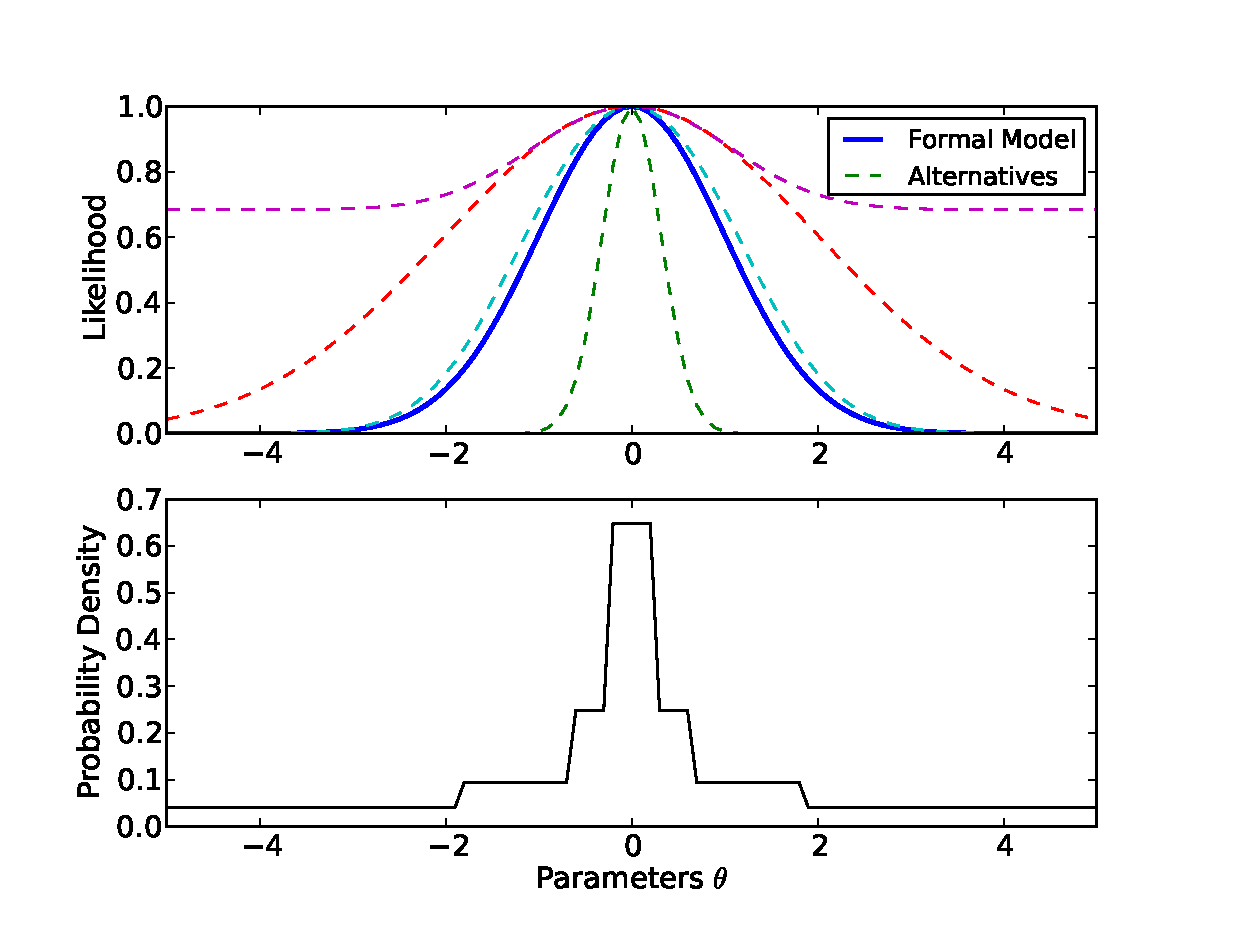
\includegraphics[scale=0.7]{nested.eps}
\end{center}
\end{figure*}

\section{More Objective Temperature Selection}
\begin{itemize}
\item If we can generate from a prior over complex models, and then fit simple models to each sample, and also generate simulated data from the complex model, we can get an idea of the joint prior over the space of (simple parameters, data)\\
\item Approximate the joint prior over (simple parameters, data) with a tempered version of the old likelihood \\
\item Find the optimal temperature that makes the approximated joint prior as close as possible to the true one.
\end{itemize}

\section{Failure Modes}
\begin{itemize}
\item If the simple model / original likelihood function is SO BAD that optimising it takes you to the wrong place in parameter space
\end{itemize}

\section{Simple Example 1: A rotation curve}

\section{Simple Example 2: An emission line}


\section{Potential Applications}

\begin{itemize}
\item Interferometry: a common goal of interferometry is to measure the angular size of some astronomical object, when it is too small to be resolved by standard telescopes. In the case of stellar interferometry, the surface brightness profile of a star is very well modelled by a circular disc with limb darkening, so this model should be used. However, with other objects, such as the dust torii in active galactic nuclei \citep[e.g.][]{2011A&A...536A..78K}, the spatial profile is not well known. If a characteristic size, or total flux or something, is the goal of the study, then the framework of this paper is applicable.\\

\item Gravitational lensing: Modelling of gravitational lenses typically aims to infer the source surface brightness profile along with the projected mass density profile of the deflector. While sophisticated many-parameter models are feasible and are used routinely now \citep{2006MNRAS.371..983S, 2007ApJ...666..726B, 2011MNRAS.412.2521B, 2006ApJ...637..608B, 2012Natur.481..341V}, they are slow, and some are not particularly realistic anyway (rant about ``regularisation'' here). With the explosion in the number of known gravitational lens systems (ref?), population-based studies will need something faster. I have already used this approach \citep{2012arXiv1201.1677B}.

\item Galaxy Structure and Morphology: Studies of populations of galaxies are often carried out by fitting simple models such as the S{\'e}rsic \citep{Sersic1968} profile to individual galaxies. It has been demonstrated that taking into account the full uncertainties on these parameters can yield different results as compared to simply studying the distribution of the best-fit parameters \citep[e.g.][]{2011MNRAS.414.1625Y}. However, since galaxies often are not well modelled by S{\'e}rsic profiles (due to their real-world complexity), the error bars on the parameters can be severely underestimated, which is almost like just using the best-fit parameters! \\

\item Studying spectra: Measuring equivalent widths, velocity dispersions and so on from emission/absorption lines. These commonly assume a specific functional form for the spectral line profile (e.g. Gaussian), which may not be applicable.

\item Any situation with correlated noise (but a believed model), we can use this method as well (e.g. \citep{2008ApJ...686..851R}).

\item Ideas? There are surely a large number of possibilities
\end{itemize}

\section*{Acknowledgements}
Tommaso Treu, Anna Pancoast, Phil Marshall, Matthew Auger, Greg Dobler, Sebastian Hoenig, Douglas Applegate


\begin{thebibliography}{99}
\bibitem[\protect\citeauthoryear{Barnab{\`e} 
\& Koopmans}{2007}]{2007ApJ...666..726B} Barnab{\`e} M., Koopmans L.~V.~E., 2007, ApJ, 666, 726 

\bibitem[\protect\citeauthoryear{Brewer 
\& Lewis}{2006}]{2006ApJ...637..608B} Brewer B.~J., Lewis G.~F., 2006, ApJ, 637, 608 

\bibitem[\protect\citeauthoryear{Brewer et al.}{2011}]{2011MNRAS.412.2521B} 
Brewer B.~J., Lewis G.~F., Belokurov V., Irwin M.~J., Bridges T.~J., Evans 
N.~W., 2011, MNRAS, 412, 2521 

\bibitem[\protect\citeauthoryear{Brewer et al.}{2012}]{2012arXiv1201.1677B} 
Brewer B.~J., et al., 2012, arXiv, arXiv:1201.1677 

\bibitem[\protect\citeauthoryear{Caticha}{2008}]{caticha} 
Caticha A., 2008, arXiv, arXiv:0808.0012 

\bibitem[\protect\citeauthoryear{Jaynes 
\& Bretthorst}{2003}]{2003prth.book.....J} Jaynes E.~T., Bretthorst G.~L., 2003, prth.book,  

\bibitem[\protect\citeauthoryear{Kishimoto et 
al.}{2011}]{2011A&A...536A..78K} Kishimoto M., H{\"o}nig S.~F., Antonucci R., Millour F., Tristram K.~R.~W., Weigelt G., 2011, A\&A, 536, A78 

\bibitem[\protect\citeauthoryear{Riechers et 
al.}{2008}]{2008ApJ...686..851R} Riechers D.~A., Walter F., Brewer B.~J., 
Carilli C.~L., Lewis G.~F., Bertoldi F., Cox P., 2008, ApJ, 686, 851 

\bibitem[{{S{\'e}rsic}(1968)}]{Sersic1968}
{S{\'e}rsic}, J.~L. 1968, {Atlas de galaxias australes} (Cordoba, Argentina:
  Observatorio Astronomico)


\bibitem[\protect\citeauthoryear{Sivia \& Skilling}{2006}]{sivia} Sivia, 
D.~ S., Skilling, J., 2006, Data Analysis: A Bayesian Tutorial, 2nd 
Edition, Oxford University Press

\bibitem[\protect\citeauthoryear{Skilling}{2006}]{skilling} Skilling, 
J., 2006, ``Nested Sampling for General Bayesian Computation'', Bayesian 
Analysis 4, pp. 833-860

\bibitem[\protect\citeauthoryear{Suyu et al.}{2006}]{2006MNRAS.371..983S} 
Suyu S.~H., Marshall P.~J., Hobson M.~P., Blandford R.~D., 2006, MNRAS, 
371, 983 

\bibitem[Richards et al.(2011)]{2011arXiv1105.6344R} Richards, J.~W., Lee, 
A.~B., Schafer, C.~M., Freeman, P.~E.\ 2011.\ Prototype selection for 
parameter estimation in complex models.\ ArXiv e-prints arXiv:1105.6344. 

\bibitem[\protect\citeauthoryear{Vegetti et 
al.}{2012}]{2012Natur.481..341V} Vegetti S., Lagattuta D.~J., McKean J.~P., 
Auger M.~W., Fassnacht C.~D., Koopmans L.~V.~E., 2012, Natur, 481, 341 

\bibitem[\protect\citeauthoryear{Yoon, Weinberg, 
\& Katz}{2011}]{2011MNRAS.414.1625Y} Yoon I., Weinberg M.~D., Katz N., 2011, MNRAS, 414, 1625 
\end{thebibliography}

\end{document}

